\documentclass[tikz,border=5mm]{standalone}
\begin{document}
	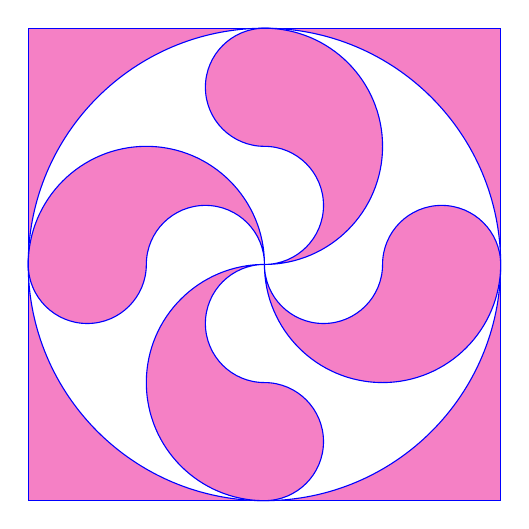
\begin{tikzpicture}[draw=blue]
		\def\a{3}  % nửa cạnh hình vuông
		\colorlet{mauto}{magenta!50!white}
		\draw[fill=mauto] (-\a,-\a) rectangle (\a,\a);
		\draw[fill=white] (0,0) circle(\a);
		\foreach \i in {0,90,180,270}
		\draw[fill=mauto,rotate=\i] (0,0) 
		arc(-180:0:\a/4) 
		arc(180:0:\a/4) 
		arc(0:-180:\a/2);
	\end{tikzpicture}

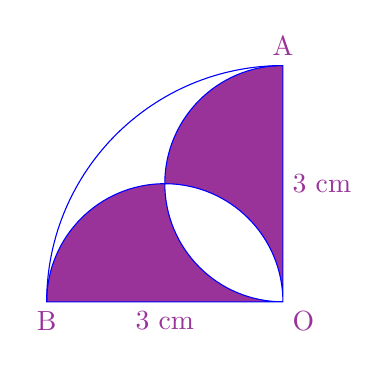
\begin{tikzpicture}
	\fill[violet!80,even odd rule,draw=blue]
	(0,0) node[below right]{O}--
	(0,3) node[above]{A} node[midway,right]{$3$ cm}
	arc(90:270:1.5)
	arc(0:180:1.5) node[below]{B}--
	cycle node[midway,below]{$3$ cm};
	\draw[blue] (0,3) arc(90:180:3);
\end{tikzpicture}

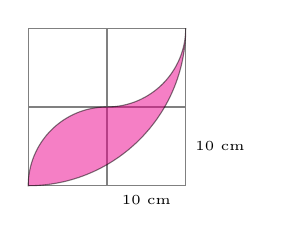
\begin{tikzpicture}
	\draw[gray] (0,0) grid (2,2);
	\draw[opacity=.5,fill=magenta] (0,0)
	arc(-90:0:2) arc(0:-90:1) arc(90:180:1)--cycle;
	\path (1,0)--
	(2,0) node[midway,below]{\tiny $10$ cm}--
	(2,1) node[midway,right]{\tiny $10$ cm};
\end{tikzpicture}

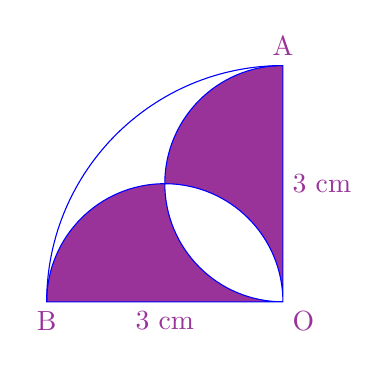
\begin{tikzpicture}
	\fill[violet!80,even odd rule,draw=blue]
	(0,0) node[below right]{O}--
	(0,3) node[above]{A} node[midway,right]{$3$ cm}
	arc(90:270:1.5)
	arc(0:180:1.5) node[below]{B}--
	cycle node[midway,below]{$3$ cm};
	\draw[blue] (0,3) arc(90:180:3);
\end{tikzpicture}

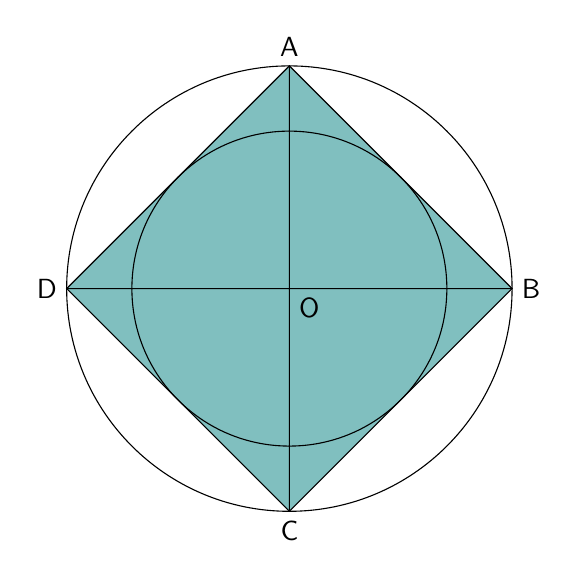
\begin{tikzpicture}[font=\sffamily]
	% các bán kính
	\def\r{2}
	\pgfmathsetmacro{\R}{\r*sqrt(2)}
	\filldraw[fill=teal!50,draw=black]
	(\R,0) node[right]{B}--
	(0,\R) node[above]{A}--
	(-\R,0) node[left]{D}--
	(0,-\R) node[below]{C}--cycle;
	\draw (0,0) node[below right]{O}
	circle(\r) circle(\R)
	(0,\R)--(0,-\R) (\R,0)--(-\R,0);
\end{tikzpicture}
\end{document}